\documentclass{beamer}
\usetheme{Warsaw}  %% Themenwahl

\usepackage{color}
\setbeamertemplate{navigation symbols}{}

\title{WearLoc}
\subtitle{Midterm presentation}
\author{L. Gemein, D. Speck, A. Biedenkapp, R. Gelhausen, J. Nist}
\date{\today}

\begin{document}
\maketitle

\begin{frame} %%Eine Folie
\frametitle{WearLoc}%%Folientitel
\begin{center}Simultaneous Localization and Mapping (SLAM)
\end{center}
\begin{figure}
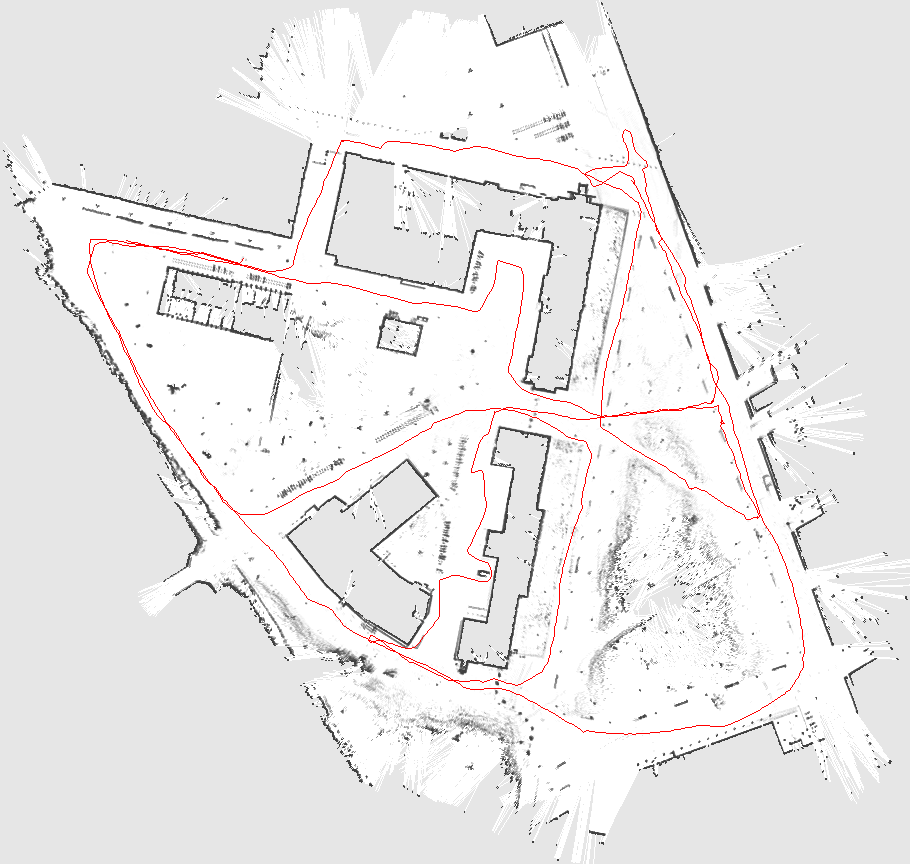
\includegraphics[width=0.5\textwidth]{slam.png} 
\caption{SLAM: \url{http://ais.informatik.uni-freiburg.de/teaching/ss15/robotics/slides/16-graph-slam.pdf}}
\end{figure}
\end{frame}


\begin{frame}
\frametitle{Schedule}
\begin{itemize}
\item \textcolor{lightgray}{\textbf{04.05.2016: Group presentations}}
\item 2 weeks: installing ROS + connecting Sensor
\item 2 weeks: prepearing data (calibrations) + writing interface
\item 1 week: time buffer 
\item \textbf{08.06.2016: Mid-Term Presentations} \\
$\Rightarrow$ all necessary data available/accessible in ROS
\color{lightgray}
\item 2 weeks: first SLAM + calibrations
\item 2 weeks: refinements + design
\item 2 weeks: time buffer
\item \textbf{20.07.2016: Final Presentations} \\
$\Rightarrow$ working WearLoc version + (live presentation) 
\end{itemize}
\end{frame}


\begin{frame}
\frametitle{Progress}
\begin{itemize}
\item Notebook running ROS kinetic 
\pause
\item Raspberry Pi running ROS indigo 
\pause
\item Working Wi-Fi connection Pi $\Leftrightarrow$ Notebook 
\pause
\item 360$^{\circ}$ Laser Scanner Rplidar attached to Pi
\pause
\item Grove IMU 9DOF attached to Pi
\pause
\item Adapted version of Hector Slam ROS package
\end{itemize}
\end{frame}


\begin{frame}
\frametitle{IMU demonstration}
\begin{figure}
\begin{center}
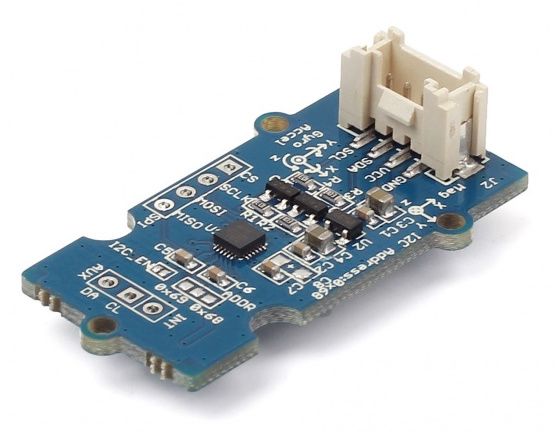
\includegraphics[width=0.5\textwidth]{IMU.JPG}
\end{center}
\end{figure}
\end{frame}


\begin{frame}
\frametitle{Prototype demonstration}
\end{frame}


\begin{frame}
\frametitle{Yet to come...}
\begin{itemize}
\item Improve map quality: better IMU calibration, different laser scanner
\pause
\item Scale it down: Intel Edison instead of Pi, smaller power bank
\pause
\item Increase operating range: eduroam instead of notebook hotspot
\pause
\item Make it acutally wearable: one-handed / no-handed design
\end{itemize}
\end{frame}


\begin{frame}
\frametitle{Yet to come...?}
\begin{itemize}
\item Include odometry information
\pause
\item 3D mapping
\pause
\item Highlight interesting map locations
\end{itemize}
\end{frame}

\end{document}